\documentclass[11pt]{article}
\usepackage[T1]{fontenc}
\usepackage[utf8]{inputenc}
\usepackage{lmodern,amsmath,amssymb,graphicx,geometry,microtype,setspace,booktabs,caption}
\usepackage[hidelinks]{hyperref}
\geometry{letterpaper,margin=1in}
\setlength{\parindent}{0pt}
\setlength{\parskip}{0.55em}
\setlength{\emergencystretch}{2em}
\captionsetup{labelfont=bf,font=small}
\renewcommand{\refname}{References}

\pagestyle{empty}
\renewcommand{\thefigure}{S\arabic{figure}}
\setcounter{figure}{5}

\begin{document}
\begin{figure}[!ht]\centering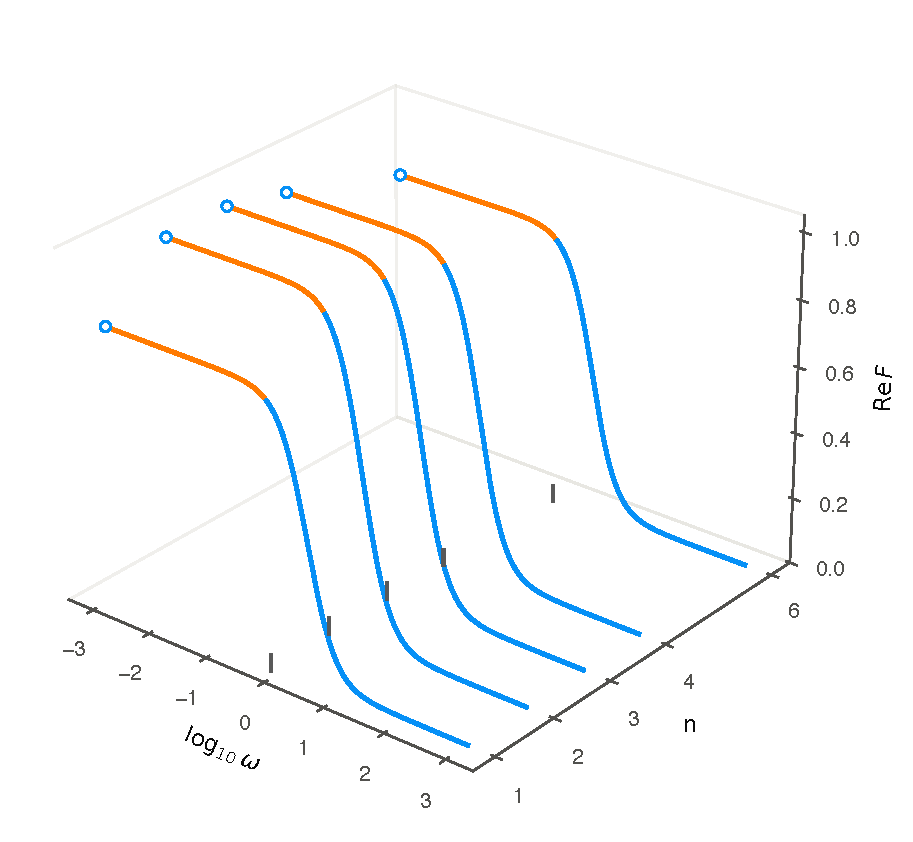
\includegraphics[width=\textwidth,height=0.65\textheight,keepaspectratio]{figure_inputs/FigS6_stability.pdf}\begin{singlespace}\caption{A frequency-domain sufficient condition under buffered-effector, fast-binding assumptions. Direct resolvent evaluation of Re F for the independent-site family specified in S13, with time in units of mean exit rate. Blue portions satisfy the analytic frequency threshold in Eq. (S34); orange portions fall below that threshold and are not classified by this bound. This convention is applied to every n. All sampled values remain positive, including below the threshold. Open circles at the left edge denote the analytic zero-frequency limits, placed there for visibility. Gray marks on the floor denote the thresholds. This is a numerical example and a partial analytic certificate, not an all-parameter stability proof.}\end{singlespace}\end{figure}
\end{document}
